\documentclass[
    tikz,
    border=5px,
    convert={
        density=600,
        size=400x400,
        outext=.svg,
        convertexe={dvisvgm},
        command=\unexpanded{{\convertexe\space --pdf  --zoom=1.5 \infile}}}]
    {standalone}

\definecolor{w}{RGB}{255,255,255}
\begin{document}
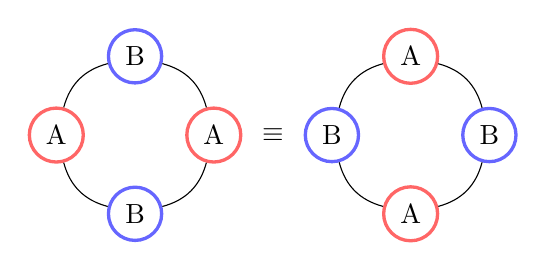
\begin{tikzpicture}[
        red/.style={circle, draw=red!60, fill=w, very thick},
        blue/.style={circle, draw=blue!60, fill=w, very thick},
        green/.style={circle, draw=green!60,  fill=w, very thick},
    ]

    \node[red] (1) at (0,0) {A};
    \node[blue] (2) at (1,1) {B};
    \node[red] (3) at (2,0) {A};
    \node[blue] (4) at (1,-1) {B};

    \path
    (1) edge[bend left, looseness=1] (2)
    (2) edge[bend left, looseness=1] (3)
    (3) edge[bend left, looseness=1] (4)
    (4) edge[bend left, looseness=1] (1)
    ;

    \node at (2.75,0) {$\equiv$};

    \node[blue] (5) at (3.5,0) {B};
    \node[red] (6) at (4.5,1) {A};
    \node[blue] (7) at (5.5,0) {B};
    \node[red] (8) at (4.5,-1) {A};

    \path
    (5) edge[bend left, looseness=1] (6)
    (6) edge[bend left, looseness=1] (7)
    (7) edge[bend left, looseness=1] (8)
    (8) edge[bend left, looseness=1] (5)
    ;
\end{tikzpicture}
\end{document}